\documentclass[11pt]{ctexart}
\usepackage[toc]{multitoc}%目录两栏
\usepackage{mathrsfs}
\usepackage{color}
\usepackage{titlesec}
\usepackage{amsmath,amsthm,amssymb}
\usepackage{amsmath}  
\usepackage{hyperref}
\usepackage{geometry}
\usepackage{graphicx}
\usepackage{appendix}
\usepackage{float}%设置图片浮动位置的宏包
\usepackage{subfig}%插入多图时用子图显示的宏包
\title{数值分析作业}
\author{CY.SP}
\date{\today}
\geometry{left=2.5cm,right=2.5cm,top=2.5cm,bottom=2.5cm}
\titleformat{\section}[block]{\centering\Large\bfseries}{\thesection}{1em}{}
\DeclareMathOperator{\li}{li}
\DeclareMathOperator{\sgn}{sgn}
\newcommand{\R}{\mathbb{R}}
\newcommand{\dx}{\mathrm{d}x}
\newcommand{\ad}{\textbf{附注}$\quad$}
\newcommand{\diam}{\mathrm{diam}}
\renewcommand{\qed}{\hfill\blacksquare}
\newcommand{\qedwhite}{\hfill \ensuremath{\Box}}
\numberwithin{equation}{subsection}
\newtheorem{theorem}{\hspace{2em}Theorem}[subsection]
\newtheorem{lemma}{\hspace{2em}Lemma}[subsection]
\newtheorem{definition}{\hspace{2em}Definition}[subsection]
\newtheorem{code}{\textbf{Code}}[subsection]
\newtheorem{ex}{\hspace{2em}Q}[subsection]
\usepackage{fontspec}
\usepackage{listings}  % 引入 listings 包
\definecolor{dkgreen}{rgb}{0,0.6,0}
\definecolor{gray}{rgb}{0.5,0.5,0.5}
\definecolor{mauve}{rgb}{0.58,0,0.82}
\lstset{
	frame=trbl,
	aboveskip=3mm,
	belowskip=3mm,
	showstringspaces=true,
	breaklines=true,
	columns=flexible,
	framerule=1pt,
	rulecolor=\color{gray},
	backgroundcolor=\color{white},
	basicstyle={\ttfamily},
	numbers=left,
	numbersep=1em,
	numberstyle=\color{black},
	keywordstyle=\color{blue},
	commentstyle=\color{gray},
	stringstyle=\color{mauve},
	tabsize=3,
}
\begin{document}
	\maketitle
	\tableofcontents
	\everymath{\displaystyle}
	\clearpage
	\section{第一周数值分析实验}
\subsection{第一节:级数求和与二元函数绘图}
\begin{ex}
编程求$\sum_{n=1}^{12}{n!}$的值.
\end{ex}
\lstinputlisting[language=matlab]{day1/work1q1.m}
\qa 522956313
\begin{ex}
绘制二元函数图像.
$$
f(x,y)=x^4-2x^2y+x^2-2xy+2y^2+\frac{9}{2}x-4y+4\,\,\,\,\left( -2\le x\le 3,-1\le y\le 7 \right) .
$$
\end{ex}
\begin{multicols}{2}
\lstinputlisting[language=matlab]{day1/work1q2.m}
\qa 
\begin{figure}[H]
	\centering
	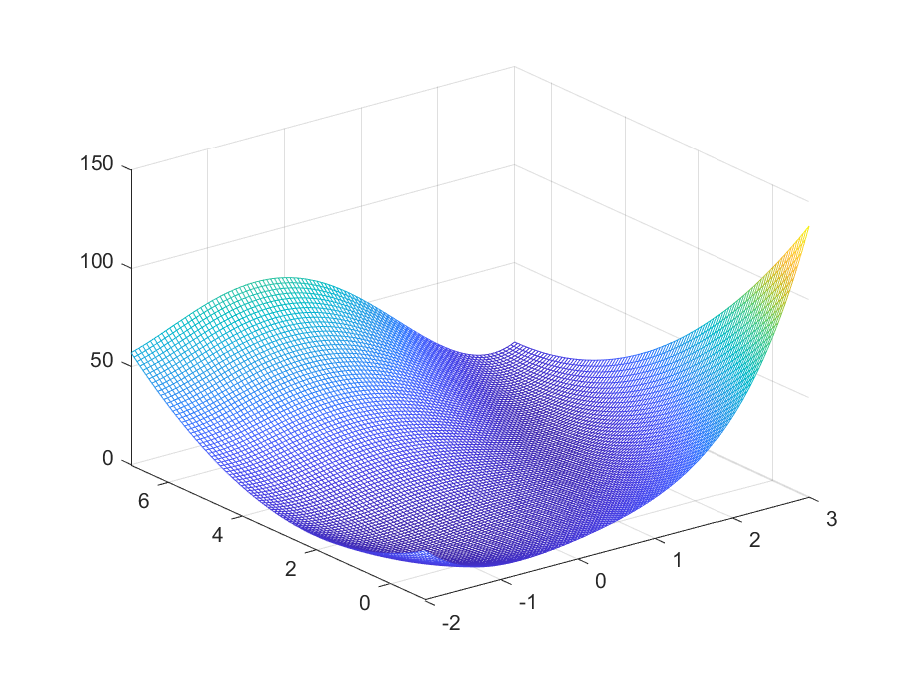
\includegraphics[width = 0.8\linewidth]{day1/q2.eps}
	\caption{运行结果}
\end{figure}
\end{multicols}
\subsection{第二节:积分递推公式}
\begin{ex}
	计算$I_n=e^{-1}\int_0^1{x^ne^xdx},(n=0,1,2,\cdots)$并估计误差
	
	方法1:利用递推公式 (A)
	$$
	\left( A \right) \text{ }\left\{ \begin{array}{l}
		I_n=1-nI_{n-1},\text{ }n=1,2,\cdots ,20\\
		I_0=1-e^{-1}\approx 0.6321.\\
	\end{array} \right. 
	$$
	
	方法2:利用递推公式 (B)
	$$
	\left( B \right) \left\{ \begin{array}{l}
		\widetilde{I_{20}}=?;\\
		\widetilde{I}_{n-1}=\frac{1}{n}\left( 1-\widetilde{I_n} \right) ,\text{ \,\,}n=19,\cdots ,9,8,\cdots 0.\\
	\end{array} \right. 
	$$
\end{ex}
\lstinputlisting[language=matlab]{day1/work1q3.m}
\qa 
% Table generated by Excel2LaTeX from sheet 'Sheet1'
\begin{table}[H]
	\centering
	\caption{运行结果}
	\resizebox{1\columnwidth}{!}{
	\begin{tabular}{|c|cccccccccc|}
		\hline
		n     & 1     & 2     & 3     & 4     & 5     & 6     & 7     & 8     & 9     & 10 \\
		IA    & 0.3679 & 0.2642 & 0.2074 & 0.1704 & 0.148 & 0.112 & 0.216 & -0.728 & 7.552 & -74.52 \\
		EA    & 5.00E-05 & 5.00E-05 & 0.0001 & 0.0003 & 0.0012 & 0.006 & 0.036 & 0.252 & 2.016 & 18.144 \\
		n     & 11    & 12    & 13    & 14    & 15    & 16    & 17    & 18    & 19    & 20 \\
		IA    & 820.72 & -9847.64 & 128020.3 & -1792283 & 26884253 & -4.3E+08 & 7.31E+09 & -1.3E+11 & 2.5E+12 & -5E+13 \\
		EA    & 181.44 & 1995.84 & 23950.08 & 311351 & 4358915 & 65383718 & 1.05E+09 & 1.78E+10 & 3.2E+11 & 6.08E+12 \\
		\hline\hline
		n     & 1     & 2     & 3     & 4     & 5     & 6     & 7     & 8     & 9     & 10 \\
		IB    & 0.367879 & 0.264241 & 0.207277 & 0.170893 & 0.145533 & 0.126802 & 0.112384 & 0.100932 & 0.091612 & 0.083877 \\
		EB    & 2.06E-20 & 4.11E-20 & 1.23E-19 & 4.93E-19 & 2.47E-18 & 1.48E-17 & 1.04E-16 & 8.29E-16 & 7.46E-15 & 7.46E-14 \\
		n     & 11    & 12    & 13    & 14    & 15    & 16    & 17    & 18    & 19    & 20 \\
		IB    & 0.077352 & 0.071773 & 0.066948 & 0.062732 & 0.059018 & 0.05572 & 0.052768 & 0.05018 & 0.04658 & 0.0684 \\
		EB    & 8.20E-13 & 9.84E-12 & 1.28E-10 & 1.79E-09 & 2.69E-08 & 4.30E-07 & 7.31E-06 & 0.000132 & 0.0025 & 0.05 \\
		\hline
	\end{tabular}%
	}
	\label{tab:addlabel1}%
\end{table}%
\begin{ex}
	计算$I_n=\int_0^1{\frac{x^n}{x+5}dx},(n=0,1,2,\cdots 20)$并估计误差.
\end{ex}
\lstinputlisting[language=matlab]{day1/work1q4.m}
\qa 
% Table generated by Excel2LaTeX from sheet 'Sheet1'
\begin{table}[H]
	\centering
	\caption{运行结果}
	\resizebox{1\columnwidth}{!}{
	\begin{tabular}{|c|cccccccccc|}
		\hline
		n     & 1     & 2     & 3     & 4     & 5     & 6     & 7     & 8     & 9     & 10 \\
		IA    & 0.0885 & 0.0575 & 0.045833 & 0.020833 & 0.095833 & -0.3125 & 1.705357 & -8.40179 & 42.12004 & -210.5 \\
		EA    & 5.00E-06 & 2.50E-05 & 0.000125 & 0.000625 & 0.003125 & 0.015625 & 0.078125 & 0.390625 & 1.953125 & 9.765625 \\
		n     & 11    & 12    & 13    & 14    & 15    & 16    & 17    & 18    & 19    & 20 \\
		IA    & 1052.592 & -5262.88 & 26314.46 & -131572 & 657861.2 & -3289306 & 16446529 & -8.2E+07 & 4.11E+08 & -2.1E+09 \\
		EA    & 48.82813 & 244.1406 & 1220.703 & 6103.516 & 30517.58 & 152587.9 & 762939.5 & 3814697 & 19073486 & 95367432 \\
		\hline\hline
		n     & 1     & 2     & 3     & 4     & 5     & 6     & 7     & 8     & 9     & 10 \\
		IB    & 0.088392 & 0.058039 & 0.043139 & 0.034306 & 0.028468 & 0.024325 & 0.021233 & 0.018837 & 0.016926 & 0.015368 \\
		EB    & 2.62E-18 & 1.31E-17 & 6.55E-17 & 3.28E-16 & 1.64E-15 & 8.19E-15 & 4.10E-14 & 2.05E-13 & 1.02E-12 & 5.12E-12 \\
		n     & 11    & 12    & 13    & 14    & 15    & 16    & 17    & 18    & 19    & 20 \\
		IB    & 0.014071 & 0.012977 & 0.01204 & 0.011229 & 0.010521 & 0.009896 & 0.009342 & 0.008846 & 0.008402 & 0.00799 \\
		EB    & 2.56E-11 & 1.28E-10 & 6.40E-10 & 3.20E-09 & 1.60E-08 & 8.00E-08 & 4.00E-07 & 2.00E-06 & 1.00E-05 & 5.00E-05 \\
		\hline
	\end{tabular}%
	}
	\label{tab:addlabel2}%
\end{table}%

	\section{第二周数值分析实验}
\subsection{第一节:插值function}
\subsubsection{直接法}
\lstinputlisting[language=matlab]{day2/Vslove.m}
\subsubsection{Lagrange法}
\lstinputlisting[language=matlab]{day2/lagrangeslove.m}
\subsection{第二节:计算实例}
\begin{ex}
	给出插值点
	$$x = (0.25, 0.3, 0.39, 0.45, 0.53, 0.66, 0.72)^T,$$  
	$$y = (0.5, 0.5477, 0.6245, 0.6708, 0.7280, 1.0254, 0.9521)^T .$$ 
	时的两种方法插值多项式表达式及对应的函数图像, 并与MATLAB拟合工具箱(cftool)进行比较.
\end{ex}
\subsubsection{直接法计算}
\lstinputlisting[language=matlab]{day2/mainvslove.m}
\subsubsection{Lagrange法计算}
\lstinputlisting[language=matlab]{day2/mainlagrange.m}
\subsubsection{结果}
\begin{figure}[H]
	\centering
	\subfloat[直接法图像]{\includegraphics[width = 0.5\linewidth]{day2/fig1.eps}}
	\hfill
	\subfloat[Lagrange法图像]{\includegraphics[width = 0.5\linewidth]{day2/fig2.eps}}
	\caption{运行结果}
	\label{fig:cj12}
\end{figure}

	\section{第三周数值分析实验}
\subsection{Newton法均差表function}
\lstinputlisting[language=matlab]{day3/newtonmatrix.m}
\subsection{\texttt{page32ex4}实例}
\lstinputlisting[language=matlab]{day3/work3.m}
\qa $y=\frac{2702819642032443\,x^5}{9223372036854775808}+\frac{2792012692852253541\,x^4}{92233720368547758080}+\frac{456060272710172342613\,x^3}{3689348814741910323200}\\+\frac{218532157850334883771\,x^2}{7378697629483820646400}+\frac{91322270122367737446143\,x}{92233720368547758080000}+\frac{146974433410736655459}{115292150460684697600000}$
\begin{figure}[H]
	\centering
	\includegraphics[width = 0.6\linewidth]{day3/newton.eps}
	\caption{Newton法结果}
\end{figure}


	\section{第四周数值分析实验}
\begin{ex}
	自行选择节点,构造插值多项式,并估计$\sqrt{2},\sqrt{2.2},\sqrt{2.5}$的值.
		不得使用牛顿切线法;不得涉及无理数运算;有效数字位数不少于$5$位.
\end{ex}
\subsection{三点三次Hermite插值}
\lstinputlisting[language=matlab]{day4/work4h33.m}
\qa [1.4142, 1.4832, 1.5811]
\subsection{两点三次Hermite插值}
\lstinputlisting[language=matlab]{day4/work4h23.m}
\qa [1.4142, 1.4833, 1.5811]
\begin{figure}[H]
	\centering
	\subfloat[三点三次Hermite插值]{\includegraphics[width = 0.5\linewidth]{day4/h33.eps}}
	\hfill
	\subfloat[两点三次Hermite插值]{\includegraphics[width = 0.5\linewidth]{day4/h23.eps}}
	\caption{运行结果}
	\label{fig:day4}
\end{figure}


	\section{第六周数值分析实验}
\subsection{Bernstein多项式}
\begin{definition}
	设$f:[0,1]\to\mathbb{R}$,称
	$$
	B_n(f;x)=\sum_{i=0}^{n}f\left(\frac{i}{n}\right)B_i^n(x),x\in[0,1]
	$$
	为$f$的$n$次Bernstein多项式,其中$B_i^n(x)=\binom{n}{i}x^i(1-x)^{n-i}$.
\end{definition}
\lstinputlisting[language=matlab]{day5/bernstein_n.m}
\begin{ex}
	当$f(x)=\cos 2\pi x$时,分别给出$n=3, 5, 7, 9, 10$时的$B_n(f,x)$表达式,并绘制$f(x)$与$B_n(f,x)$的图像.
\end{ex}
\lstinputlisting[language=matlab]{day5/work6.m}
\qa 

\begin{flalign*}
	&B_3(f,x)=\frac{9\,x^2}{2}-\frac{9\,x}{2}+1.&
\end{flalign*}
\begin{flalign*}
	\begin{split}
		B_5(f,x)=&-\frac{17396110258977045\,x^4}{2251799813685248}+\frac{69584441035908185\,x^3}{4503599627370496}\\&-\frac{19232666484692435\,x^2}{4503599627370496}-\frac{3889888508315415\,x}{1125899906842624}+1.
	\end{split}&
\end{flalign*}
\begin{flalign*}
	\begin{split}
		B_7(f,x)=&\frac{7\,x^7}{36028797018963968}+\frac{48511846945173955\,x^6}{18014398509481984}-\frac{291071081671043793\,x^5}{36028797018963968}\\&-\frac{39777928968693195\,x^4}{9007199254740992}+\frac{100417737650160665\,x^3}{4503599627370496}-\frac{22201645688437845\,x^2}{2251799813685248}\\&-\frac{11869558316351393\,x}{4503599627370496}+1.
	\end{split}&
\end{flalign*}
\begin{flalign*}
	\begin{split}
		B_9(f,x)=&-\frac{63\,x^9}{2251799813685248}-\frac{3651501963845295\,x^8}{9007199254740992}+\frac{912875490961461\,x^7}{562949953421312}\\&+\frac{4844390630064489\,x^6}{1125899906842624}-\frac{41846600653847829\,x^5}{2251799813685248}+\frac{21573830928373101\,x^4}{4503599627370496}\\&+\frac{26215294559596821\,x^3}{1125899906842624}-\frac{29056921947987975\,x^2}{2251799813685248}-\frac{18965558858231295\,x}{9007199254740992}+1.
	\end{split}&
\end{flalign*}
\begin{flalign*}
	\begin{split}
		B_{10}(f,x)=&\frac{36617051598889\,x^{10}}{4503599627370496}-\frac{183085257994425\,x^9}{4503599627370496}-\frac{1745013596718105\,x^8}{2251799813685248}\\&+\frac{3764655080427825\,x^7}{1125899906842624}+\frac{16286793569370555\,x^6}{4503599627370496}-\frac{51167254958838837\,x^5}{2251799813685248}\\&+\frac{42639379132365645\,x^4}{4503599627370496}+\frac{25803329789012535\,x^3}{1125899906842624}-\frac{15656499233079345\,x^2}{1125899906842624}\\&-\frac{1075138741208855\,x}{562949953421312}+1.
	\end{split}&
\end{flalign*}

\begin{figure}[H]
	\centering
	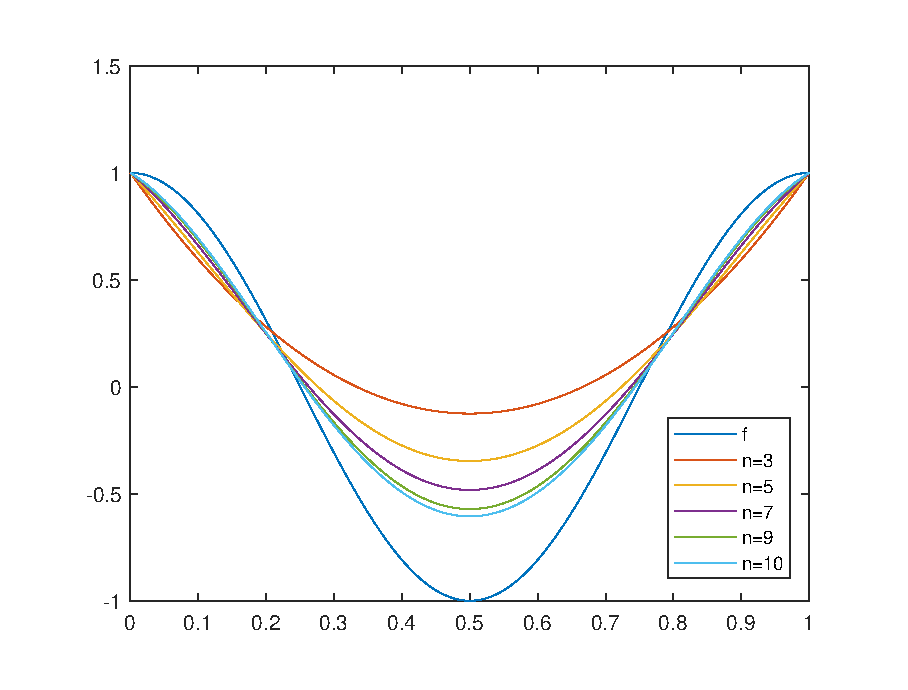
\includegraphics[width = 0.6\linewidth]{day5/fig.eps}
	\caption{Bernstein多项式图像}
\end{figure}
	\section{第六周数值分析实验}

\end{document}